% Options for packages loaded elsewhere
\PassOptionsToPackage{unicode}{hyperref}
\PassOptionsToPackage{hyphens}{url}
\PassOptionsToPackage{dvipsnames,svgnames*,x11names*}{xcolor}
%
\documentclass[
  fontsize=13pt,
  english,
  a4paper,
  openany, a4paper, oneside]{article}
\usepackage{amsmath,amssymb}
\usepackage{lmodern}
\usepackage{setspace}
\usepackage{ifxetex,ifluatex}
\ifnum 0\ifxetex 1\fi\ifluatex 1\fi=0 % if pdftex
  \usepackage[T1]{fontenc}
  \usepackage[utf8]{inputenc}
  \usepackage{textcomp} % provide euro and other symbols
\else % if luatex or xetex
  \usepackage{unicode-math}
  \defaultfontfeatures{Scale=MatchLowercase}
  \defaultfontfeatures[\rmfamily]{Ligatures=TeX,Scale=1}
\fi
% Use upquote if available, for straight quotes in verbatim environments
\IfFileExists{upquote.sty}{\usepackage{upquote}}{}
\IfFileExists{microtype.sty}{% use microtype if available
  \usepackage[]{microtype}
  \UseMicrotypeSet[protrusion]{basicmath} % disable protrusion for tt fonts
}{}
\makeatletter
\@ifundefined{KOMAClassName}{% if non-KOMA class
  \IfFileExists{parskip.sty}{%
    \usepackage{parskip}
  }{% else
    \setlength{\parindent}{0pt}
    \setlength{\parskip}{6pt plus 2pt minus 1pt}}
}{% if KOMA class
  \KOMAoptions{parskip=half}}
\makeatother
\usepackage{xcolor}
\IfFileExists{xurl.sty}{\usepackage{xurl}}{} % add URL line breaks if available
\IfFileExists{bookmark.sty}{\usepackage{bookmark}}{\usepackage{hyperref}}
\hypersetup{
  pdftitle={Open Collaboration Guide},
  pdfauthor={Daniel Antal},
  pdflang={en},
  colorlinks=true,
  linkcolor=blue,
  filecolor=Maroon,
  citecolor=Blue,
  urlcolor=blue,
  pdfcreator={LaTeX via pandoc}}
\urlstyle{same} % disable monospaced font for URLs
\usepackage[left=3cm, right=3cm, top=2.5cm, bottom=2.5cm]{geometry}
\usepackage{color}
\usepackage{fancyvrb}
\newcommand{\VerbBar}{|}
\newcommand{\VERB}{\Verb[commandchars=\\\{\}]}
\DefineVerbatimEnvironment{Highlighting}{Verbatim}{commandchars=\\\{\}}
% Add ',fontsize=\small' for more characters per line
\usepackage{framed}
\definecolor{shadecolor}{RGB}{248,248,248}
\newenvironment{Shaded}{\begin{snugshade}}{\end{snugshade}}
\newcommand{\AlertTok}[1]{\textcolor[rgb]{0.94,0.16,0.16}{#1}}
\newcommand{\AnnotationTok}[1]{\textcolor[rgb]{0.56,0.35,0.01}{\textbf{\textit{#1}}}}
\newcommand{\AttributeTok}[1]{\textcolor[rgb]{0.77,0.63,0.00}{#1}}
\newcommand{\BaseNTok}[1]{\textcolor[rgb]{0.00,0.00,0.81}{#1}}
\newcommand{\BuiltInTok}[1]{#1}
\newcommand{\CharTok}[1]{\textcolor[rgb]{0.31,0.60,0.02}{#1}}
\newcommand{\CommentTok}[1]{\textcolor[rgb]{0.56,0.35,0.01}{\textit{#1}}}
\newcommand{\CommentVarTok}[1]{\textcolor[rgb]{0.56,0.35,0.01}{\textbf{\textit{#1}}}}
\newcommand{\ConstantTok}[1]{\textcolor[rgb]{0.00,0.00,0.00}{#1}}
\newcommand{\ControlFlowTok}[1]{\textcolor[rgb]{0.13,0.29,0.53}{\textbf{#1}}}
\newcommand{\DataTypeTok}[1]{\textcolor[rgb]{0.13,0.29,0.53}{#1}}
\newcommand{\DecValTok}[1]{\textcolor[rgb]{0.00,0.00,0.81}{#1}}
\newcommand{\DocumentationTok}[1]{\textcolor[rgb]{0.56,0.35,0.01}{\textbf{\textit{#1}}}}
\newcommand{\ErrorTok}[1]{\textcolor[rgb]{0.64,0.00,0.00}{\textbf{#1}}}
\newcommand{\ExtensionTok}[1]{#1}
\newcommand{\FloatTok}[1]{\textcolor[rgb]{0.00,0.00,0.81}{#1}}
\newcommand{\FunctionTok}[1]{\textcolor[rgb]{0.00,0.00,0.00}{#1}}
\newcommand{\ImportTok}[1]{#1}
\newcommand{\InformationTok}[1]{\textcolor[rgb]{0.56,0.35,0.01}{\textbf{\textit{#1}}}}
\newcommand{\KeywordTok}[1]{\textcolor[rgb]{0.13,0.29,0.53}{\textbf{#1}}}
\newcommand{\NormalTok}[1]{#1}
\newcommand{\OperatorTok}[1]{\textcolor[rgb]{0.81,0.36,0.00}{\textbf{#1}}}
\newcommand{\OtherTok}[1]{\textcolor[rgb]{0.56,0.35,0.01}{#1}}
\newcommand{\PreprocessorTok}[1]{\textcolor[rgb]{0.56,0.35,0.01}{\textit{#1}}}
\newcommand{\RegionMarkerTok}[1]{#1}
\newcommand{\SpecialCharTok}[1]{\textcolor[rgb]{0.00,0.00,0.00}{#1}}
\newcommand{\SpecialStringTok}[1]{\textcolor[rgb]{0.31,0.60,0.02}{#1}}
\newcommand{\StringTok}[1]{\textcolor[rgb]{0.31,0.60,0.02}{#1}}
\newcommand{\VariableTok}[1]{\textcolor[rgb]{0.00,0.00,0.00}{#1}}
\newcommand{\VerbatimStringTok}[1]{\textcolor[rgb]{0.31,0.60,0.02}{#1}}
\newcommand{\WarningTok}[1]{\textcolor[rgb]{0.56,0.35,0.01}{\textbf{\textit{#1}}}}
\usepackage{longtable,booktabs,array}
\usepackage{calc} % for calculating minipage widths
% Correct order of tables after \paragraph or \subparagraph
\usepackage{etoolbox}
\makeatletter
\patchcmd\longtable{\par}{\if@noskipsec\mbox{}\fi\par}{}{}
\makeatother
% Allow footnotes in longtable head/foot
\IfFileExists{footnotehyper.sty}{\usepackage{footnotehyper}}{\usepackage{footnote}}
\makesavenoteenv{longtable}
\setlength{\emergencystretch}{3em} % prevent overfull lines
\providecommand{\tightlist}{%
  \setlength{\itemsep}{0pt}\setlength{\parskip}{0pt}}
\setcounter{secnumdepth}{5}
\usepackage{booktabs}
\usepackage{amsthm}
\makeatletter
\def\thm@space@setup{%
  \thm@preskip=8pt plus 2pt minus 4pt
  \thm@postskip=\thm@preskip
}
\makeatother
\ifxetex
  % Load polyglossia as late as possible: uses bidi with RTL langages (e.g. Hebrew, Arabic)
  \usepackage{polyglossia}
  \setmainlanguage[]{english}
\else
  \usepackage[main=english]{babel}
% get rid of language-specific shorthands (see #6817):
\let\LanguageShortHands\languageshorthands
\def\languageshorthands#1{}
\fi
\ifluatex
  \usepackage{selnolig}  % disable illegal ligatures
\fi
\usepackage[]{natbib}
\bibliographystyle{apalike}

\title{Open Collaboration Guide}
\author{Daniel Antal}
\date{2021-03-27}

\begin{document}
\maketitle

{
\hypersetup{linkcolor=}
\setcounter{tocdepth}{2}
\tableofcontents
}
\setstretch{1.1}
\hypertarget{welcome}{%
\section*{Welcome}\label{welcome}}
\addcontentsline{toc}{section}{Welcome}

\texttt{I\ didn\textquotesingle{}t\ have\ time\ to\ write\ a\ short\ letter,\ so\ I\ wrote\ a\ long\ one\ instead.} --- \emph{Mark Twain}

For collaborators who do not write code, the general \protect\hyperlink{intro}{Introduction} contains a \protect\hyperlink{simple-intro}{Simple Introduction} focusing on documentation tools only. Contributors with no coding experience and ambition will likely work with \protect\hyperlink{data-curation}{data curation} and \protect\hyperlink{documentation}{documentation, publications} which is equally important to developing code. You must be familiar with our developers \protect\hyperlink{naming-conventions}{naming conventions}, because we automate research: their programs create data tables, visualizations, maps, blogposts, even books following this vocabulary.

Most of this long-form documentation is intended for collaborators who write code to \protect\hyperlink{acquisition}{acquire data}, \protect\hyperlink{data-storage}{store data}, create applications such a \protect\hyperlink{statistical-software}{statistics}, or \protect\hyperlink{machine-learning}{machine learning applications}, and who help us \protect\hyperlink{data-release}{publish data}.

Open collaboration is an agile project management method that breaks up the tasks to small, independent, decentralized acts that can be performed by individuals or research groups. It requires a solid shared knowledge base and a very high quality documentation. This collaboration guide serves two goals: to practice this documentation workflow, and to create a continuously improved documentation for our collaboration methods and practices.

\hypertarget{intro}{%
\section{Introduction}\label{intro}}

Provided that you use whatever IDE and Git/Github, there is unlikely that this guide will pose any challenge for you. Markdown and YAML are very simple, special-purpose markdown ``languages'' (the language is a big word here) that you can learn in 1-2 hours. They create marked up text, which we use for a hypertextual reference guide.

To collaboration on our software data products, there are other skills necessary, but for documentation and publication, technically you can get started with a clean text editor and git. We have a \protect\hyperlink{simple-intro}{Simplified Introduction} for you, which shows what can you skip in the rest of the document -- almost everything. But do not skip this \protect\hyperlink{intro}{Introduction}.

\hypertarget{definitions}{%
\subsection{Definitions}\label{definitions}}

\begin{itemize}
\item
  \texttt{Open\ Data} is data that is freely available to everyone to use and republish without legal or other restrictions. The most important sources of open data are open science data connected to scientific activities that allow the replication of scientific achievements. In Europe, the re-use of public sector information, in other jurisdictions, freedom of information regulations make various public institutions' and taxpayer funded datasets available for reuse. Open data is a very important source of information for business, scientific and policy uses.
\item
  \texttt{Reproducible\ research}: The quality control of open data is focusing on reviewable, reproducible and confirmable findings. Auditability is a requirement in most high-level business, scientific or policy applications.
\item
  \texttt{Open\ Source}: In most cases, when the data processing code and procedure is not a well-documented, open-source algorithm, reproducibility and confirmability is limited, or impossible.
\item
  \texttt{Metadata}: It is a means by which the complexity of an object is represented in a simpler form. For example, the title, the author, and the cover art are metadata about a book. We use the distinction of descriptive, administrative, structural, preservation, and use metadata. See \protect\hyperlink{metadata}{metadata}.
\end{itemize}

\hypertarget{code-of-conduct}{%
\subsection{Code of Conduct}\label{code-of-conduct}}

We as members, contributors, and leaders pledge to make participation in our
community a harassment-free experience for everyone, regardless of age, body
size, visible or invisible disability, ethnicity, sex characteristics, gender
identity and expression, level of experience, education, socio-economic status,
nationality, personal appearance, race, caste, color, religion, or sexual identity and orientation.

We pledge to act and interact in ways that contribute to an open, welcoming,
diverse, inclusive, and healthy community.

*If you work with us, you must adhere to the \protect\hyperlink{covenant}{Contributor Covenant Code of Conduct}

\hypertarget{collaboration-tools}{%
\subsection{Collaboration Tools}\label{collaboration-tools}}

\hypertarget{keybase}{%
\subsubsection{Instant messaging: Keybase}\label{keybase}}

Keybase is a very neat, simple, lightweight team management / chat / social networking application that is extremely focused on privacy, security and encryption.

\textbf{Keybase Key features}

\begin{itemize}
\item
  Secure instant messaging, even with a timed self-destruction feature (e.g.~for sharing passwords);
  Starts a Google Meet or Zoom video call natively with a single command;
\item
  Brings your Whatsapp chat to the more private and secure keybase chat on the fly;
\item
  Team chat rooms in real time. You can filter where you want to be involved, and you can always opt-out;
\end{itemize}

-K-Drive (similar to OneDrive, Google Drive, Dropbox) -- only for our team, and fully encrypted;
Works with Github, and it even offers a more private version of Private Github Repos, encrypted gits;
An integration with other platforms;
It is neat, open source, simple, clean, and usually appreciated more in the open source community than Slack, its big corporation rival.

Practical steps you need to follow to use Keybase

\begin{enumerate}
\def\labelenumi{\arabic{enumi}.}
\tightlist
\item
  Download \& install Keybase from \url{https://keybase.io/} on your computer.
\end{enumerate}

An easy procedure. Create yourself a professional login name -- similarly to a professional github account, a professional email, etc. (you cannot change the name afterwards)

\begin{enumerate}
\def\labelenumi{\arabic{enumi}.}
\setcounter{enumi}{1}
\item
  Once you log in to the computer, go to \emph{Devices}, and \emph{Create a paper key}. Write this on paper, or print it, and store it somewhere very safe (not near your computer). This to recover the access in case you lose access to all your devices.
\item
  You can use Keybase simultaneously on multiple devices -- Install Keybase on your smartphone, tablet or any other device. You will be guided through installation \& paired with your computer.
\item
  Shall you need them, you have \emph{two recovery options}: the paper key and your smartphone.
\item
  If your smartphone breaks down and needs a replacement, you can add from your computer your new phone and deactivate the old one.
\item
  Once you are in, look up \texttt{antaldaniel}. (Daniel is antaldaniel on Facebook, Twitter, Instagram, github, gmail, yahoo and basically every place where he was an early user, so you can connect with him on whatever channel you want.)
\item
  After a handshake Daniel will assist your smooth transition, help you find ways to our shared files, your project's files, and set up filters, so you are not flooded with information, while never left out, unless you choose to.
\item
  Initially, we set up the following ``Big teams'', as Keybase calls them, and we will send an invitation to join:
\end{enumerate}

\begin{itemize}
\tightlist
\item
  \texttt{reprexscience} for our data science teams;
\item
  \texttt{reprexdev} for developer(s), which may overlap with business development and science;
\item
  \texttt{reprexbd} for business development, which may overlap with science;
\item
  \texttt{reprexhumanities} for our creative team and data journalism
\item
  \texttt{reprexfriends} for prospective team members, friends, and hoped-for-cooperation partners -- partly for people we are discreetly asking to join us, or who want to know more about some of our work and cooperate with us;
\item
  \texttt{reprexmanagement} for Istvan (general management) and Daniel (co-founder) - this is a closed team for now;
\item
  \texttt{reprexmusic20} for our Music Professionals 2020 team.
\item
  \href{https://keybase.io/team/reprexcommunity}{reprexcommunity} is an open landing page for anybody, it is a public interface. If you every land there \texttt{antaldaniel} will take you to the appropriate, otherwise invisible team room.
\end{itemize}

Each big team has four special members for a smooth transition: Daniel and Zuzana to assist you with getting familiar with Keybase, zoombot (just type \texttt{!zoom} to create a Zoom call with the team members present) and meetbot (that does the same with Google Meet, \texttt{!meet}). Daniel will gradually withdraw from some of the teams, once their support is not needed, though each team will have at least one Reprex co-founder present. We invite everybody to at least one team, but you can sign up to as many as you like, shall you find that convenient.

\begin{enumerate}
\def\labelenumi{\arabic{enumi}.}
\setcounter{enumi}{8}
\tightlist
\item
  Whenever you are in a situation you want to ignore us (e.g.~because you sit in your dayjob), just do it. If you have a smartphone, we are there, separated from your Whatsapp friends, work emails, and you can always check on us. We can always send you a secure (and even encrypted) message to get in touch, if needed. However, we will never ever bother you with long emails, Whatsapp messages and other annoying things.
\end{enumerate}

\emph{Let's keep things short, give access to the full picture when needed, and let you find out what mix of response time, details and filters works best for you.}

\hypertarget{github}{%
\subsubsection{Git \& Github}\label{github}}

Git is a simultaneous collaboration for for any distributed team work - writing, programming, design work. Git is an open source software which makes sure that your teamwork files are always synchronized, clashes are avoided (you modify the same part of a file at the same time with Daniel.) The only hard part to move to Git is to make sure that Git properly works on your computer - it needs to be installed differently on all Linux distros, Mac OSX version all Windows versions. On Windows, you must make sure that Git is on the startup path. Once you are there, you'll life will be much easier.

\begin{itemize}
\item
  \protect\hyperlink{keybase}{Keybase} allows the group work on encrypted documents, like business proposals simultaneously using Git synch.
\item
  RStudio allows us to work simultaneously on business proposals, blog posts, templates via Git.
\item
  Github is allows us to use shared folders (\texttt{repositories} or simply \texttt{repos}) where we can track changes, modify the same thing at the same time, avoid or resolve conflicting edits, assign tasks, and much more.
\end{itemize}

If you do not have a github account yet, please, sign up now on \href{https://github.com/}{github.com}. Create a very professional profile. It is likely that you will use this profile for future works for decades, as Git is really becoming the norm of digital nomads, freelancers, and tech teams to work together.

Github is not the only service platform that allows distributed, collaborative teamwork. It has many alternatives, for example, GitLab -- don't confuse them. We use Github.

\begin{itemize}
\tightlist
\item
  \href{https://github.com/dataobservatory-eu}{dataobservatory-eu} is our private repo collection and private github collaboration platform.
\end{itemize}

\hypertarget{rstudio-ide-other-ide}{%
\subsubsection{Rstudio IDE \& other IDE}\label{rstudio-ide-other-ide}}

Our recommended IDE for documentation purposes is RStudio. You must install R, RStudio at least to make it work. For PDF outputs, you need to add a pdf compiler (recommended: tinytex, a lightweight tex compiler.) If you want to run Python code within RStudio, you need to have Pyhton installed on your computer, too. If you work in documentation and publishing, think about RStudio as a word processor that can save your work in html, pdf, Word, epub, keynote, PowerPoint, or any OpenOffice or Apple formats.

We work with data in the R and Python language, and we are open for C++, too. Our documentation is made in markdown to be able to produce html, pdf, word, powerpoint, reveal.js or any type of output. Our long-form documentation is knit together with the help of the `bookdown', `knitr', `rmarkdown' packages in the R language -- they combine YAML headers and enriched markdown that can contain R, Python or C++ executable code `chunks', and our website use markdown, hugo, and the `blogdown' connector between Go, R, and markdown.

This heterogeneous workflow is best served in RStudio. While you can write code in your favorite IDE in Python and/or C++, RStudio is unrivaled in its capability to connect various markup languages and several programming languages. Therefore, for documentation purposes, we use RStudio. You can contribute in any other editor -- our longform documentation and our website content is, after all, marked-up text. If you need to execute something for within the documentation, only RStudio will do the trick.

\hypertarget{simple-intro}{%
\subsection{Simple Introduction}\label{simple-intro}}

\begin{quote}
This part is intendend for collaborators who do not write regularly code, and do not use markdown, LaTeX in their work.
\end{quote}

You will likely work with \protect\hyperlink{data-curation}{data curation} and \protect\hyperlink{documentation}{documentation, publications} which is equally important to developing code.

\hypertarget{markdown}{%
\subsubsection{Markdown}\label{markdown}}

Markdown is a simple ``language'', or rather a writing notation system that lets the word processor know that \texttt{*italics*} means \emph{italics}, or \texttt{**bold**} means \textbf{bold} or \texttt{\#\#\ Writing,\ blogging} becomes a level 2 heading, and \texttt{\#\#\#\ Markdown\ \{\#markdown\}} is a level 3 heading that can be referenced in the table of contents or internal hypertext links with \texttt{{[}Jump\ to\ markdown\ introduction{]}(\#markdown)}.

Markdown makes it possible that we can work on documents that will render fine in \texttt{html}, \texttt{docs}, \texttt{pptx}, \texttt{pdf}, \texttt{google\ docs}, or \texttt{md} for markdown files.

Markdown is a ``markup language''. But that is a too big word. It is more of a notation system for writing clear text that later can be automatically formatted.

For example \texttt{{[}Introduction\ to\ RMarkdown{]}(https://rmarkdown.rstudio.com/lesson-1.html)} creates the hypertext link \href{https://rmarkdown.rstudio.com/lesson-1.html}{Introduction to RMarkdown} in \texttt{html}, \texttt{docs}, \texttt{pptx}, \texttt{pdf}, \texttt{iWork\ Keynote}, \texttt{xlsx} or any file format that we need to create.

Markdown is very important for reproducible research and automation. It makes sure that the content and the form is fully separated.

\begin{itemize}
\item
  It is always the computer's task to make the formatting work perfectly and beautifully.
\item
  It is sometimes the computer's task to fill out the document with text and numbers.
\item
  It is a human task to desnbng beautiful documents, like blogposts, business proposals, research reports that are very easy to replicate automatically.
\end{itemize}

Markdown is not strictly a language, and it has many `flavors' or notation version. The differences are usually related to the programming interface that allows the file conversion. If you are new to markdown, you can start with any flavor, the main text functions are the same.

\begin{itemize}
\item
  \href{https://stackedit.io/}{StackEdit} is a wonderful tool, and we would recommend it, if it would not have been suspended from the Google Drive integration. You can try it out online. It is probably the cleanest interface to get you started.
\item
  \href{https://thumbsdb.herokuapp.com/markdown/}{Heroku Markdown Editor} integrates reasonably easily to your Google Drive. This means that you can edit our blogposts in your Google Documents.
\item
  \href{https://gsuite.google.com/marketplace/app/docs_to_markdown/700168918607}{Docs to Markdown} translates your Google Docs to Markdown. However, you must link your own images via a valid path.
\item
  \href{https://rstudio.com/}{RStudio} is our preferred offline application. It integrates seamlessly with Github. It is an integrated programming environment with four panels. If you use it as a markdown text editor, you can just minimize or close the programming tools.
\end{itemize}

RStudio uses the Rmarkdown, a special version of markdown, where you can insert little programs in \texttt{R}, \texttt{Python}, \texttt{C++}, \texttt{SQL}, \texttt{D3} or \texttt{Bash} scripts. For example, you can write a blogpost that retrieves data with a little program written by our musicology team from Spotify, or embeds a YouTube video, etc. The \texttt{code\ chunks} are visually separated from the proposal or blog post text, and you can ignore it if you do not \emph{yet} write code.

\begin{itemize}
\tightlist
\item
  \href{https://rstudio.com/wp-content/uploads/2016/03/rmarkdown-cheatsheet-2.0.pdf?_ga=2.126386957.1623649708.1603024238-59012930.1603024238}{RMarkdown Cheat Sheet}
\item
  \href{https://rstudio.com/wp-content/uploads/2015/03/rmarkdown-reference.pdf?_ga=2.68348561.1623649708.1603024238-59012930.1603024238}{Rmarkdown Reference}
\end{itemize}

\hypertarget{inspiration}{%
\subsection{Inspiration \& Recommended Reading}\label{inspiration}}

\hypertarget{books}{%
\subsubsection{Books}\label{books}}

\hypertarget{why-weapons-of-math-destruction}{%
\paragraph{Why: Weapons of Math Destruction}\label{why-weapons-of-math-destruction}}

Weapons of math destruction, which O'Neil refers to throughout the book as WMDs, are mathematical models or algorithms that claim to quantify important traits: teacher quality, recidivism risk, creditworthiness but have harmful outcomes and often reinforce inequality, keeping the poor poor and the rich rich. They have three things in common: opacity, scale, and damage \citep{weapons_of_math_destruction}.

\url{https://blogs.scientificamerican.com/roots-of-unity/review-weapons-of-math-destruction/}

\hypertarget{how-metadata}{%
\paragraph{How: Metadata}\label{how-metadata}}

Metadata describes all the information that we collect, storeand disseminate in the forms of tables, maps, charts, apps, articles and books. Metadata is not data, it is the organization of data that is ready for use, publication, archiving or other purposes.

We follow the metadata definition and concepts of \href{https://mitpress.mit.edu/books/metadata}{Pomerantz: Metadata} from the MIT Press Essential Knowledge series \citep{pomerantz_2015}. If you are a data scientist or an engineer, you will understand this book well. If you help us with data journalism, documentation, publications, this small book can help you understand the challenges we face when we want to make sure that our data will be easy to find, easy to use, transparent with the ``small print.'' Read this short book by just skipping whatever you find technical. The first chapters of the book will save you countless of hours of misunderstandings.

It is not, Pomerantz tell us, just ``data about data.'' It is a means by which the complexity of an object is represented in a simpler form. For example, the title, the author, and the cover art are metadata about a book. When metadata does its job well, it fades into the background; everyone (except perhaps the NSA) takes it for granted.

\hypertarget{critically-data-feminism}{%
\paragraph{Critically: Data Feminism}\label{critically-data-feminism}}

Critical attitude to working with with big data and AI: \href{https://mitpressonpubpub.mitpress.mit.edu/data-feminism}{Data Feminism}. This is a much celebrated book, and with a good reason. It views AI and data problems with a feminist point of view, but the examples and the toolbox can be easily imagined for small-country biases, racial, ethnic, or small enterprise problems. A very good introduction to the injustice of big data and the fight for a more fair use of data \citep{data_feminism}.

\hypertarget{blogposts}{%
\subsubsection{Blog posts \& Podcasts}\label{blogposts}}

``big data increases inequality and threatens democracy.'' With Facebook's new \href{http://qz.com/769413/heres-how-facebooks-automated-trending-bar-probably-works/}{trending topics algorithm} and \href{https://medium.com/equal-future/predictive-policing-is-happening-now-and-police-could-learn-a-real-lesson-from-minority-report-e105a592eda0\#.h90q9xoqx}{data-driven policing} in the news, the book is certainly timely.

Any single episode of the now discontinued What's the Point Podcast: \url{https://fivethirtyeight.com/features/introducing-fivethirtyeight-newest-podcast-whats-the-point/}

\begin{itemize}
\item
  How a bad algorithm re-organized fire stations that hurt the black Bronx the most when the fire broke out: \href{https://fivethirtyeight.com/features/why-the-bronx-really-burned/}{Why The Bronx Really Burned}
\item
  \href{https://fivethirtyeight.com/features/whos-accountable-when-an-algorithm-makes-a-bad-decision/}{Who's Accountable When An Algorithm Makes A Bad Decision?} Cathy O'Neil is most interested in meet three criteria: They are widespread, secret and unfair --- the scoring methods that she says, for example, generate credit scores, keep someone in prison, or deny someone a job. On this week's What's The Point, O'Neil discusses her new book, ``\href{https://weaponsofmathdestructionbook.com/}{Weapons of Math Destruction}''
\item
  In \href{https://nyupress.org/9781479837243/algorithms-of-oppression/}{Algorithms of Oppression}, Safiya Umoja Noble challenges the idea that search engines like Google offer an equal playing field for all forms of ideas, identities, and activities. Data discrimination is a real social problem; Noble argues that the combination of private interests in promoting certain sites, along with the monopoly status of a relatively small number of Internet search engines, leads to a biased set of search algorithms that privilege whiteness and discriminate against people of color, specifically women of color. - submitted by \href{https://keybase.io/ajgmolina}{ajgmolina}
\end{itemize}

\hypertarget{data-curation}{%
\section{Data Curation}\label{data-curation}}

We are constantly looking for new data sources that may be interesting to our partners or for our own R\&D activities.

\hypertarget{acquisition}{%
\section{Data Acquistion}\label{acquisition}}

Whatever is the source of the data we use it, we never trust it fully. We need check its strength and weaknesses, and bring it to a complete, documented and tidy form.

\hypertarget{collect-metadata}{%
\subsection{Metadata}\label{collect-metadata}}

Metadata plays an important role to find whatever we acquired and use it properly. It plays an important role during the storage of data in our \protect\hyperlink{data-storage}{databases} and in \protect\hyperlink{documentation}{documentation and publication}, too. We placed it into a \protect\hyperlink{metadata}{separate chapter}.

\hypertarget{eurostat}{%
\subsection{Eurostat}\label{eurostat}}

\hypertarget{harmonized-survey-programs}{%
\subsection{Harmonized Survey Programs}\label{harmonized-survey-programs}}

\hypertarget{music-apis}{%
\subsection{Music APIs}\label{music-apis}}

\hypertarget{spotify-api}{%
\subsubsection{Spotify API}\label{spotify-api}}

\hypertarget{bandcamp}{%
\subsubsection{Bandcamp}\label{bandcamp}}

\hypertarget{data-storage}{%
\section{Data Storage \& Databases}\label{data-storage}}

We may pursue several data storage philosophies.

Sometimes it is best to download data as it is, without processing, and saving it. These are the raw data assets. The raw data can be stored in a file system, or a very simple database.

Often it is not desirable to save the data in raw form, and we pre-process it to limit redundancy. For example, when downloading data from the Spotify API, it may be desirable to filter out redundant information, and just save marginal, new data. This data is best stored in some searchable, amendable database.

When we work with machine learning applications, we usually need tidy and processed individual data. When we work with business, policy, scientific analysis, we often need statistically aggregated (or disaggregated) data. Similarly to a machine learning application, the individual data goes through a complicated and error-prone software code until it gains its final form. The best view for a non-statistical data scientist to view our indicator creation process as an app itself. When we release a regional GDP dataset, we modify the input data in a very complicated process, and the published dataset is not an input (like a well-designed feature set) but a finished output.

The finished statistical output is a product, not a raw ingredient, and it is not desirable to store it in a database format. There are so many things that can go wrong with an indicator. Our statistical indicators are created by a code that is never finished. Whenever a new issue comes up, we add more processing code, new unit-tests. We constantly improve the statistically processed datasets, they need versioning, and often the best solution if the raw data is processed on the spot with the latest code.

We resisted databases for long, particularly centralized databases, because statistical end-products are at best created instantaneously with the best available data input, processing code and unit-testing.

Placing data in a database, particularly a not very well documented database goes against our core reproducible research principles. Strictly speaking, we must reveal our entire data process, from downloading a data point from the Spotify API to releasing a visualization, both input and processing code. A database adds a lot of complexity and renders the full process oversight unreadable. While technically reproducability may still be there, it is not inviting. (We can also reverse-engineer a lot of data processes, but we do not think that this is a real reproducible practice.)

We always must keep the right balance between the advantages of using a database and the advantages of a fully transparent and readable data workflow. We must balanace the documentation burden of a constantly updated database with keeping the process as a documentation and not hiding immediate results in a database.

\hypertarget{storage-metadata}{%
\subsection{Metadata}\label{storage-metadata}}

Metadata plays an important role in our \protect\hyperlink{data-storage}{databases} and in \protect\hyperlink{documentation}{documentation}, too. We placed it into a \protect\hyperlink{metadata}{separate chapter}.

\hypertarget{dta-raw}{%
\subsection{Raw data assets}\label{dta-raw}}

\hypertarget{processed-individual-data}{%
\subsection{Processed, individual data}\label{processed-individual-data}}

\hypertarget{indicators---statistically-processed-data}{%
\subsection{Indicators - statistically processed data}\label{indicators---statistically-processed-data}}

\hypertarget{periodic-data-releases}{%
\subsection{Periodic data releases}\label{periodic-data-releases}}

\hypertarget{interactive-data-releases}{%
\subsection{Interactive data releases}\label{interactive-data-releases}}

\hypertarget{continous-data-releases-in-api}{%
\subsection{Continous data releases in API}\label{continous-data-releases-in-api}}

\hypertarget{applications}{%
\section{Applications}\label{applications}}

We process and release data to be used in various business, policy and scientific applications. In this collaboration guideline we do not want to document these applications - they are very specific to the problem, domain or client. The aim of this guideline to make the data collection, processing and dissemination workflow open for collaborators. The aim of this collaboration is to create high-quality, timely and well-documented data assets for various applications. We add application-specific information here to the extent that it helps data collaboration.

\hypertarget{naming-conventions}{%
\subsection{File, Variable Names, Value Labels}\label{naming-conventions}}

\begin{quote}
There are only two hard things in Computer Science: cache invalidation and naming things. -- Phil Karlton
\end{quote}

We are mainly naming things when we name a path to a file (subdirectory and filename), create a database schema, and write code in any language. Of course, computers can translate between names, but the worst use of our time is to write code to rename things in a database to our code, or rename file names.

In recent reproducible science practice there have been many attempts to standardize variable naming. Because different (programming) languages have different well-established cultures, and naming things is a cognitive process, a full harmonization is not possible, but a high-level of harmonization already can save many-many hours in code writing, analysis and debugging.

\hypertarget{path}{%
\subsubsection{Path}\label{path}}

Because our final output is often an automatically created website (in the go language, using the hugo server application), we must be very aware of the entire path. A hugo website contains that website metadata in the path - the relative position of a file tells the server what is the aim of the file.

Our repos follow the naming conventions of peer-reviewed R packages. They can be extended to allow Python-specific elements.

Always present:
\texttt{data-raw}: subfolder that contains data to be further processed
\texttt{data}: contains well-processed, well-documented, re-usable, or publishable, releasable data.
\texttt{R}: R scripts
\texttt{plots}: saved static plots, maps
\texttt{Python}: Python scripts
\texttt{not\_included}: your scrap files, environment files, \emph{not to be synchronized on github}.

In R software releases only:
\texttt{man} : not always present, \texttt{manual} code documentation files.
\texttt{vignette}: only in R software releases, documentation file

In longform documentation only:
\texttt{\_book}: Only present in long-form bookdown publication, the current version of the books in different folders. (It is accompanied with a \texttt{\_bookdown\_files} folder)
s.

In websites only:
Hugo has its own relative path system.

\hypertarget{R-guide}{%
\paragraph{R language}\label{R-guide}}

Consider the two identical meaning R code:

\begin{Shaded}
\begin{Highlighting}[]
\FunctionTok{read.csv}\NormalTok{(}\StringTok{"data/my{-}csv.csv"}\NormalTok{)}

\FunctionTok{read.csv}\NormalTok{(}\FunctionTok{file.path}\NormalTok{(}\StringTok{"data{-}raw"}\NormalTok{, }\StringTok{"my{-}csv.csv"}\NormalTok{))}
\end{Highlighting}
\end{Shaded}

On CRAN, only the latter is permissible for publication? Why? Because the various Linux distributions, Windows and Mac uses paths differently. You can never be sure that a file path will mean the same thing with 100\% certainty, especially in the case of a full path. The full path is file-system dependent, and the three families of operational system use different ones.

The function \texttt{file.path()} in R makes sure that on any R-supported platforms your code will thy to read \texttt{my-csv.csv} from the relative \texttt{data-raw} path.

\hypertarget{variable-nameing-styles}{%
\subsubsection{Variable nameing styles}\label{variable-nameing-styles}}

We prefer the \texttt{snake\_case\_naming\_convention} with lowercase letters. The names should omit stopwords, whenever possible, remain as short as possible. The organization of the name should help simple variable name selection rules, such as \texttt{starts\_with()} or \texttt{ends\_with()} in the tidyverse - this helps programming a great deal!

Consider the following scenario:

\texttt{spotify\_artist\_id}
\texttt{spotify\_song\_id}
\texttt{spotify\_artist\_name}
\texttt{deezer\_song\_id}
\texttt{deezer\_artist\_name}
\texttt{bandcamp\_song\_id}
\texttt{bandcamp\_artist\_name}
\texttt{bandcamp\_song\_title}

Do you work with bandcamp data only:

\texttt{select\ (\ starts\_with("bandcamp"))}

Do you want to check how ID's match

\texttt{select\ (\ ends\_with("id"))}

Do you want to work with artist (person) data or song (sound recording) data as a unit?

\texttt{select\ (\ contains("song"))}

\texttt{select\ (\ contains("artist"))}

In R, we use \texttt{dbplyr} and the \texttt{tidyverse}, particularly \texttt{dplyr}, a non-standard evaluation of the language which makes R and SQL as interchangeable as possible. The \texttt{dbplyr} package allows the combination of queries to a database in SQL, R-dpylr, or even both in the same query.

Again, when updating/querying a database, the best if database columns need not to be renamed in the updating/processing code.

The \texttt{lower\_snake\_case} is a partly subjective choice. The lowercase is usually a very natural compromise between \texttt{UPPERCASE}, or \texttt{camelCase} naming conventions, and the renaming can happen with simple programmatic ways. In the R language we use the package \texttt{snakecase} for this, which translates a text or caption to any case you want - title case, camel case, snake case.

\hypertarget{character-coding}{%
\subsubsection{Character coding}\label{character-coding}}

Character coding is an unresolved problem of the world. We use \texttt{UTF-8} whatever it means, and we pray that our products will be readable on all platforms.

\hypertarget{statistical-software}{%
\subsection{Statistical Processing \& Indicators}\label{statistical-software}}

All our critical processing code goes through anonymous peer-review on CRAN. We take pride in the fact that our software goes through dozens of unit-tests and a human review and it can be tested by anybody.

\hypertarget{retroharmonize}{%
\subsubsection{retroharmonize}\label{retroharmonize}}

The aim of \href{https://reprex.nl/software/retroharmonize/}{retroharmonize} is to provide tools for reproducible retrospective (ex-post) harmonization of datasets that contain variables measuring the same concepts but coded in different ways. Ex-post data harmonization enables better use of existing data and creates new research opportunities. For example, harmonizing data from different countries enables cross-national comparisons, while merging data from different time points makes it possible to track changes over time. \citep{R-retroharmonize}

It has two peer-reviewed releases.

\hypertarget{regions}{%
\subsubsection{regions}\label{regions}}

The \href{https://reprex.nl/software/regions/}{regions} package is an offspring of the eurostat package on \href{https://github.com/rOpenGov}{rOpenGov}. It started as a tool to validate and re-code regional Eurostat statistics, but it aims to be a general solution for all sub-national statistics. It will be developed parallel with other rOpenGov packages. \citep{R-regions}

It has one peer-reviewed release.

\hypertarget{iotables}{%
\subsubsection{iotables}\label{iotables}}

\href{https://reprex.nl/software/iotables/}{iotables} processes all the symmetric input-output tables of the EU member states, and calculates direct, indirect and induced effects, multipliers for GVA, employment, taxation. These are important inputs into policy evaluation, business forecasting, or granting/development indicator design. iotables is used by about 800 experts around the world. \citep{R-iotables}

It has several peer-reviewed releases.

\hypertarget{machine-learning}{%
\subsection{Machine Learning Applications}\label{machine-learning}}

\hypertarget{listen-local-app}{%
\subsubsection{Listen Local app}\label{listen-local-app}}

\hypertarget{bandcamp-librarian-app}{%
\subsubsection{Bandcamp Librarian app}\label{bandcamp-librarian-app}}

\hypertarget{documentation}{%
\section{Documentation And Publications}\label{documentation}}

\hypertarget{citations-bibliography}{%
\subsection{Citations, Bibliography}\label{citations-bibliography}}

For any external literature, data source, please, store the citation information in a well-formatted, thematic \texttt{.bib} files.

We create programatically \texttt{.bib} citation information files for our data products, software releases, and published documents.

\begin{Shaded}
\begin{Highlighting}[]
\SpecialCharTok{@}\NormalTok{Manual\{R}\SpecialCharTok{{-}}\NormalTok{regions,}
\NormalTok{  title }\OtherTok{=}\NormalTok{ \{regions}\SpecialCharTok{:}\NormalTok{ Processing Regional Statistics\},}
\NormalTok{  author }\OtherTok{=}\NormalTok{ \{Daniel Antal\},}
\NormalTok{  note }\OtherTok{=}\NormalTok{ \{R package version }\DecValTok{0}\NormalTok{.}\FloatTok{1.6}\NormalTok{\},}
\NormalTok{  url }\OtherTok{=}\NormalTok{ \{https}\SpecialCharTok{:}\ErrorTok{//}\NormalTok{regions.danielantal.eu}\SpecialCharTok{/}\NormalTok{\},}
\NormalTok{  year }\OtherTok{=}\NormalTok{ \{}\DecValTok{2021}\NormalTok{\},}
\NormalTok{\}}

\SpecialCharTok{@}\NormalTok{Manual\{R}\SpecialCharTok{{-}}\NormalTok{retroharmonize,}
\NormalTok{  title }\OtherTok{=}\NormalTok{ \{retroharmonize}\SpecialCharTok{:}\NormalTok{ Ex Post Survey Data Harmonization\},}
\NormalTok{  author }\OtherTok{=}\NormalTok{ \{Daniel Antal\},}
\NormalTok{  note }\OtherTok{=}\NormalTok{ \{R package version }\DecValTok{0}\NormalTok{.}\FloatTok{1.15}\NormalTok{\},}
\NormalTok{  url }\OtherTok{=}\NormalTok{ \{https}\SpecialCharTok{:}\ErrorTok{//}\NormalTok{retroharmonize.dataobservatory.eu}\SpecialCharTok{/}\NormalTok{\},}
\NormalTok{  year }\OtherTok{=}\NormalTok{ \{}\DecValTok{2021}\NormalTok{\},}
\NormalTok{\}}
\end{Highlighting}
\end{Shaded}

Marking up a reference to \citep{R-retroharmonize} with \texttt{{[}@R-retroharmonize{]}} will place the citation in your selected format (here APA) to the text, and to the \protect\hyperlink{references}{references} at the end of this documentation.

\hypertarget{software-releases}{%
\subsection{Software Releases}\label{software-releases}}

We have so far three released software products.

\begin{itemize}
\tightlist
\item
  The aim of \href{https://reprex.nl/software/retroharmonize/}{retroharmonize} is to provide tools for reproducible retrospective (ex-post) harmonization of datasets that contain variables measuring the same concepts but coded in different ways.
\item
  The \href{https://reprex.nl/software/regions/}{regions} package is an offspring of the eurostat package on \href{https://github.com/rOpenGov}{rOpenGov}. It started as a tool to validate and re-code regional Eurostat statistics, but it aims to be a general solution for all sub-national statistics. It will be developed parallel with other rOpenGov packages.
\item
  \href{https://reprex.nl/software/iotables/}{iotables} processes all the symmetric input-output tables of the EU member states, and calculates direct, indirect and induced effects, multipliers for GVA, employment, taxation. These are important inputs into policy evaluation, business forecasting, or granting/development indicator design. iotables is used by about 800 experts around the world.
\end{itemize}

They are released on CRAN, and they follow the CRAN guidelines for unit-testing and human review. As CRAN relies on extensive automated testing, the formatting standard is \emph{very strict} both for the software code and its documentation. The slightest deviation results in rejection.

\hypertarget{documentation-metadata}{%
\subsection{Metadata}\label{documentation-metadata}}

Metadata plays an important role in our \protect\hyperlink{data-storage}{databases} and in \protect\hyperlink{documentation}{documentation}, too. We placed it into a \protect\hyperlink{metadata}{separate chapter}.

\hypertarget{data-release}{%
\subsection{Data releases}\label{data-release}}

We currently work with two platforms, and we must maintain compatibility with data repositories that our clients use. Both provide some validation, version control, and give a standard \textbf{doi} to our releases.

\hypertarget{dataverse}{%
\subsubsection{Dataverse}\label{dataverse}}

\href{https://dataverse.org/}{dataverse.org/} has a well-supported API, and this is the choice of our first academic partner, IViR.

The Dataverse Project is being developed at Harvard's Institute for Quantitative Social Science (IQSS), along with many collaborators and contributors worldwide. The Dataverse Project was built on our experience with our earlier Virtual Data Center (VDC) project, which spanned 1997-2006 as a collaboration between the Harvard-MIT Data Center (now part of IQSS) and the Harvard University Library. Precursors to the VDC date to 1987, comprising such entities as pre-web software to automatically transfer cataloging information by FTP to other sites across campus automatically at designated times, and before that to a stand-alone software guide to local data.

\hypertarget{zenodo}{%
\subsubsection{Zenodo}\label{zenodo}}

\href{https://zenodo.org/}{zenodo} is the choice of the European Union, and it is likely that in the future all EU-financed research data must be published here.

The OpenAIRE project, in the vanguard of the open access and open data movements in Europe was commissioned by the EC to support their nascent Open Data policy by providing a catch-all repository for EC funded research. CERN, an OpenAIRE partner and pioneer in open source, open access and open data, provided this capability and Zenodo was launched in May 2013.

In support of its research programme CERN has developed tools for Big Data management and extended Digital Library capabilities for Open Data. Through Zenodo these Big Science tools could be effectively shared with the long-tail of research.

\hypertarget{publications}{%
\subsection{Publications}\label{publications}}

Our work is often embedded in publications. We want to make the application of various formatting guidelines as painless as possible. This is one of the main motivations to use markdown and Rmarkdown to document our work. There are more and more conversion tools that automatically convert our longform documentation from markdown or Rmarkdown to the formatting standards of almost any scientific publisher.

\hypertarget{metadata}{%
\section{Metadata}\label{metadata}}

We follow the metadata definition and concepts of \href{https://mitpress.mit.edu/books/metadata}{Metadata} from the MIT Press Essential Knowledge series.

It is not, Pomerantz tell us, just ``data about data.'' It is a means by which the complexity of an object is represented in a simpler form. For example, the title, the author, and the cover art are metadata about a book. When metadata does its job well, it fades into the background; everyone (except perhaps the NSA) takes it for granted.

Pomerantz explains what metadata is, and why it exists. He distinguishes among different types of metadata---descriptive, administrative, structural, preservation, and use---and examines different users and uses of each type. He discusses the technologies that make modern metadata possible, and he speculates about metadata's future. By the end of the book, readers will see metadata everywhere. Because, Pomerantz warns us, it's metadata's world, and we are just living in it.

\hypertarget{covenant}{%
\section{Contributor Covenant Code of Conduct}\label{covenant}}

\hypertarget{our-pledge}{%
\subsection{Our Pledge}\label{our-pledge}}

We as members, contributors, and leaders pledge to make participation in our
community a harassment-free experience for everyone, regardless of age, body
size, visible or invisible disability, ethnicity, sex characteristics, gender
identity and expression, level of experience, education, socio-economic status,
nationality, personal appearance, race, caste, color, religion, or sexual identity and orientation.

We pledge to act and interact in ways that contribute to an open, welcoming,
diverse, inclusive, and healthy community.

\hypertarget{our-standards}{%
\subsection{Our Standards}\label{our-standards}}

Examples of behavior that contributes to a positive environment for our
community include:

\begin{itemize}
\tightlist
\item
  Demonstrating empathy and kindness toward other people
\item
  Being respectful of differing opinions, viewpoints, and experiences
\item
  Giving and gracefully accepting constructive feedback
\item
  Accepting responsibility and apologizing to those affected by our mistakes,
  and learning from the experience
\item
  Focusing on what is best not just for us as individuals, but for the
  overall community
\end{itemize}

Examples of unacceptable behavior include:

\begin{itemize}
\tightlist
\item
  The use of sexualized language or imagery, and sexual attention or
  advances of any kind
\item
  Trolling, insulting or derogatory comments, and personal or political attacks
\item
  Public or private harassment
\item
  Publishing others' private information, such as a physical or email
  address, without their explicit permission
\item
  Other conduct which could reasonably be considered inappropriate in a
  professional setting
\end{itemize}

\hypertarget{enforcement-responsibilities}{%
\subsection{Enforcement Responsibilities}\label{enforcement-responsibilities}}

Community leaders are responsible for clarifying and enforcing our standards of
acceptable behavior and will take appropriate and fair corrective action in
response to any behavior that they deem inappropriate, threatening, offensive,
or harmful.

Community leaders have the right and responsibility to remove, edit, or reject
comments, commits, code, wiki edits, issues, and other contributions that are
not aligned to this Code of Conduct, and will communicate reasons for moderation
decisions when appropriate.

\hypertarget{scope}{%
\subsection{Scope}\label{scope}}

This Code of Conduct applies within all community spaces, and also applies when
an individual is officially representing the community in public spaces.
Examples of representing our community include using an official e-mail address,
posting via an official social media account, or acting as an appointed
representative at an online or offline event.

\hypertarget{enforcement}{%
\subsection{Enforcement}\label{enforcement}}

Instances of abusive, harassing, or otherwise unacceptable behavior may be
reported to the community leaders responsible for enforcement at
{[}INSERT CONTACT METHOD{]}.
All complaints will be reviewed and investigated promptly and fairly.

All community leaders are obligated to respect the privacy and security of the
reporter of any incident.

\hypertarget{enforcement-guidelines}{%
\subsection{Enforcement Guidelines}\label{enforcement-guidelines}}

Community leaders will follow these Community Impact Guidelines in determining
the consequences for any action they deem in violation of this Code of Conduct:

\hypertarget{correction}{%
\subsubsection{1. Correction}\label{correction}}

\textbf{Community Impact}: Use of inappropriate language or other behavior deemed
unprofessional or unwelcome in the community.

\textbf{Consequence}: A private, written warning from community leaders, providing
clarity around the nature of the violation and an explanation of why the
behavior was inappropriate. A public apology may be requested.

\hypertarget{warning}{%
\subsubsection{2. Warning}\label{warning}}

\textbf{Community Impact}: A violation through a single incident or series
of actions.

\textbf{Consequence}: A warning with consequences for continued behavior. No
interaction with the people involved, including unsolicited interaction with
those enforcing the Code of Conduct, for a specified period of time. This
includes avoiding interactions in community spaces as well as external channels
like social media. Violating these terms may lead to a temporary or
permanent ban.

\hypertarget{temporary-ban}{%
\subsubsection{3. Temporary Ban}\label{temporary-ban}}

\textbf{Community Impact}: A serious violation of community standards, including
sustained inappropriate behavior.

\textbf{Consequence}: A temporary ban from any sort of interaction or public
communication with the community for a specified period of time. No public or
private interaction with the people involved, including unsolicited interaction
with those enforcing the Code of Conduct, is allowed during this period.
Violating these terms may lead to a permanent ban.

\hypertarget{permanent-ban}{%
\subsubsection{4. Permanent Ban}\label{permanent-ban}}

\textbf{Community Impact}: Demonstrating a pattern of violation of community
standards, including sustained inappropriate behavior, harassment of an
individual, or aggression toward or disparagement of classes of individuals.

\textbf{Consequence}: A permanent ban from any sort of public interaction within
the community.

\hypertarget{attribution}{%
\subsection{Attribution}\label{attribution}}

This Code of Conduct is adapted from the \href{https://www.contributor-covenant.org}{Contributor Covenant},
version 2.0, available at
\url{https://www.contributor-covenant.org/version/2/0/code_of_conduct.html}.

Community Impact Guidelines were inspired by
\href{https://github.com/mozilla/diversity}{Mozilla's code of conduct enforcement ladder}.

For answers to common questions about this code of conduct, see the FAQ at
\url{https://www.contributor-covenant.org/faq}. Translations are available
at \url{https://www.contributor-covenant.org/translations}.

\hypertarget{appendix}{%
\section{Appendix}\label{appendix}}

\hypertarget{markdown-1}{%
\subsection{Markdown}\label{markdown-1}}

This is a \emph{sample} book written in \textbf{Markdown}. You can use anything that Pandoc's Markdown supports, e.g., a math equation \(a^2 + b^2 = c^2\).

\hypertarget{bookdown}{%
\subsection{Bookdown}\label{bookdown}}

The \textbf{bookdown} package can be installed from CRAN or Github:

\begin{Shaded}
\begin{Highlighting}[]
\FunctionTok{install.packages}\NormalTok{(}\StringTok{"bookdown"}\NormalTok{)}
\CommentTok{\# or the development version}
\CommentTok{\# devtools::install\_github("rstudio/bookdown")}
\end{Highlighting}
\end{Shaded}

Remember each Rmd file contains one and only one chapter, and a chapter is defined by the first-level heading \texttt{\#}.

You can label chapter and section titles using \texttt{\{\#label\}} after them, e.g., we can reference Chapter \ref{intro}. If you do not manually label them, there will be automatic labels anyway, e.g., Chapter \ref{methods}.

Figures and tables with captions will be placed in \texttt{figure} and \texttt{table} environments, respectively.

\begin{Shaded}
\begin{Highlighting}[]
\FunctionTok{par}\NormalTok{(}\AttributeTok{mar =} \FunctionTok{c}\NormalTok{(}\DecValTok{4}\NormalTok{, }\DecValTok{4}\NormalTok{, .}\DecValTok{1}\NormalTok{, .}\DecValTok{1}\NormalTok{))}
\FunctionTok{plot}\NormalTok{(pressure, }\AttributeTok{type =} \StringTok{\textquotesingle{}b\textquotesingle{}}\NormalTok{, }\AttributeTok{pch =} \DecValTok{19}\NormalTok{)}
\end{Highlighting}
\end{Shaded}

\begin{figure}

{\centering 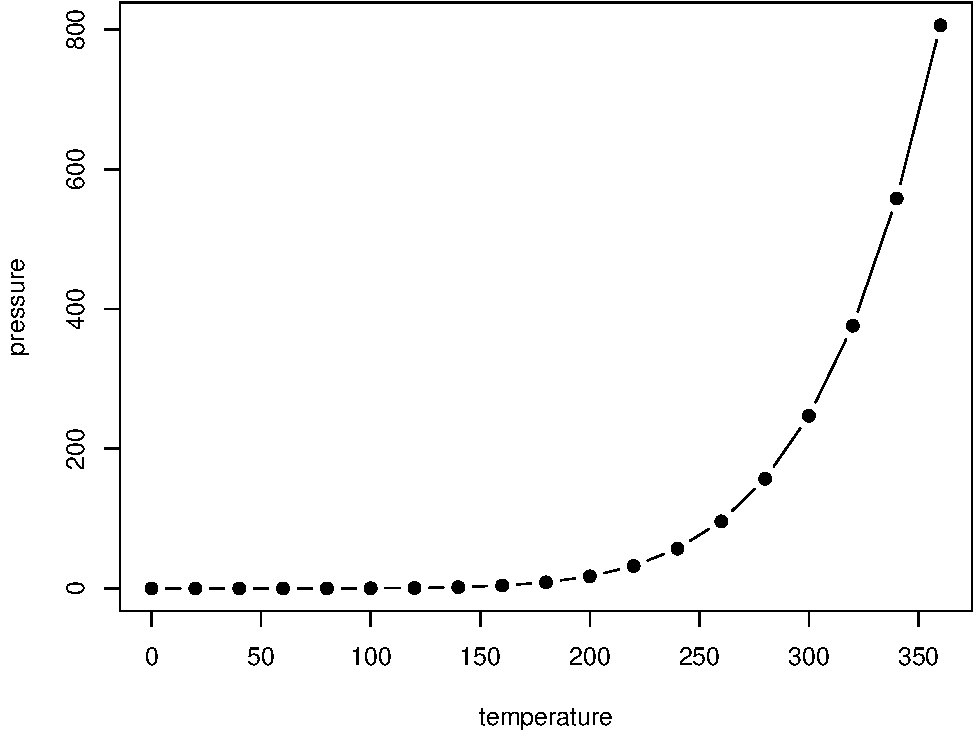
\includegraphics[width=0.8\linewidth]{reprex_collaboration_guide_files/figure-latex/nice-fig-1} 

}

\caption{Here is a nice figure!}\label{fig:nice-fig}
\end{figure}

Reference a figure by its code chunk label with the \texttt{fig:} prefix, e.g., see Figure \ref{fig:nice-fig}. Similarly, you can reference tables generated from \texttt{knitr::kable()}, e.g., see Table \ref{tab:nice-tab}.

\begin{Shaded}
\begin{Highlighting}[]
\NormalTok{knitr}\SpecialCharTok{::}\FunctionTok{kable}\NormalTok{(}
  \FunctionTok{head}\NormalTok{(iris, }\DecValTok{20}\NormalTok{), }\AttributeTok{caption =} \StringTok{\textquotesingle{}Here is a nice table!\textquotesingle{}}\NormalTok{,}
  \AttributeTok{booktabs =} \ConstantTok{TRUE}
\NormalTok{)}
\end{Highlighting}
\end{Shaded}

\begin{table}

\caption{\label{tab:nice-tab}Here is a nice table!}
\centering
\begin{tabular}[t]{rrrrl}
\toprule
Sepal.Length & Sepal.Width & Petal.Length & Petal.Width & Species\\
\midrule
5.1 & 3.5 & 1.4 & 0.2 & setosa\\
4.9 & 3.0 & 1.4 & 0.2 & setosa\\
4.7 & 3.2 & 1.3 & 0.2 & setosa\\
4.6 & 3.1 & 1.5 & 0.2 & setosa\\
5.0 & 3.6 & 1.4 & 0.2 & setosa\\
\addlinespace
5.4 & 3.9 & 1.7 & 0.4 & setosa\\
4.6 & 3.4 & 1.4 & 0.3 & setosa\\
5.0 & 3.4 & 1.5 & 0.2 & setosa\\
4.4 & 2.9 & 1.4 & 0.2 & setosa\\
4.9 & 3.1 & 1.5 & 0.1 & setosa\\
\addlinespace
5.4 & 3.7 & 1.5 & 0.2 & setosa\\
4.8 & 3.4 & 1.6 & 0.2 & setosa\\
4.8 & 3.0 & 1.4 & 0.1 & setosa\\
4.3 & 3.0 & 1.1 & 0.1 & setosa\\
5.8 & 4.0 & 1.2 & 0.2 & setosa\\
\addlinespace
5.7 & 4.4 & 1.5 & 0.4 & setosa\\
5.4 & 3.9 & 1.3 & 0.4 & setosa\\
5.1 & 3.5 & 1.4 & 0.3 & setosa\\
5.7 & 3.8 & 1.7 & 0.3 & setosa\\
5.1 & 3.8 & 1.5 & 0.3 & setosa\\
\bottomrule
\end{tabular}
\end{table}

You can write citations, too. For example, we are using the \textbf{bookdown} package \citep{R-bookdown} in this sample book, which was built on top of R Markdown and \textbf{knitr} \citep{xie2015}.

\hypertarget{tinytex}{%
\subsection{Tinytex}\label{tinytex}}

To compile this example to PDF, you need XeLaTeX. You are recommended to install TinyTeX (which includes XeLaTeX): \url{https://yihui.name/tinytex/}.

  \bibliography{book.bib,packages.bib,antal.bib,ccipolicy.bib}

\end{document}
